\section{Algorithm: choosing when and what to query}
\label{sec:async}

% Restate our goal
As described in \sectionref{model}, we would like to select and schedule several requests for labels to maximize our accuracy on predictions while trading off the cost and response time. 
We view the problem in the Bayesian decision theoretic setting: what is the optimal behavioral policy under our current beliefs?
The delay in the information we receive from label requests requires us to reason about time and the possible interactions between the responses we will receive.
In this section, we describe how these interactions can be described using an expectimax tree.
However, evaluating the optimal policy from the expectimax tree is intractable.
We propose a Monte Carlo search based algorithm to efficiently approximate the optimal policy.

% Input and output to the section
% input: model, examples.
% output: behavior policy

\begin{figure}
  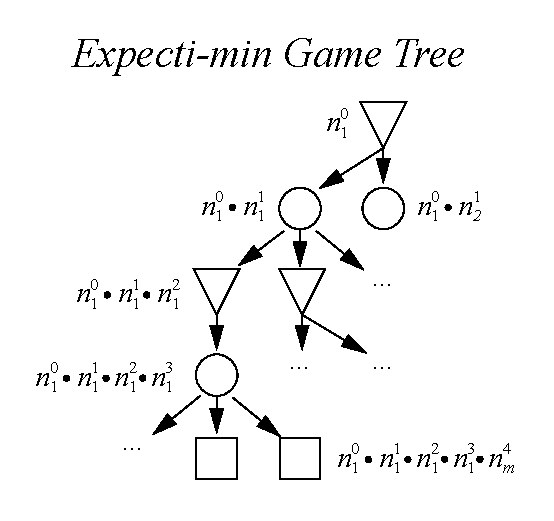
\includegraphics[width=0.49\textwidth,height=0.23\textheight,keepaspectratio]{figures/game-tree.pdf}
  \hfill
  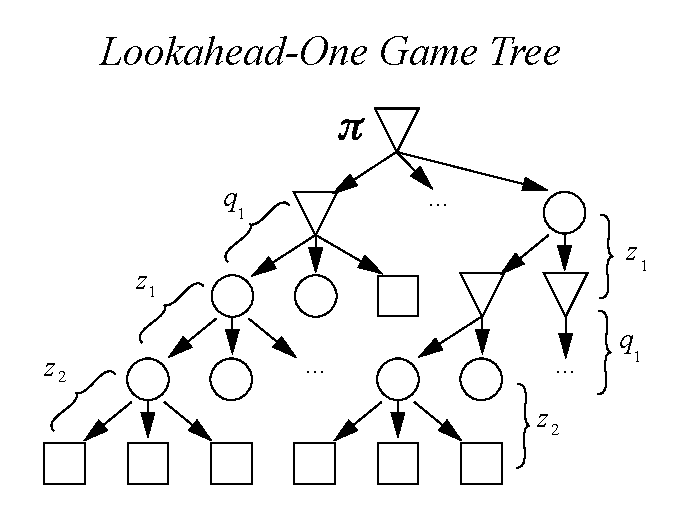
\includegraphics[width=0.49\textwidth,height=0.23\textheight,keepaspectratio]{figures/lookahead-one.pdf}
  \caption{Monte Carlo tree search}
\label{fig:mcts}
\end{figure}

For each input example $\bx$, we construct an expectimax tree (\figureref{mcts} left) as follows: 
\begin{itemize}
  \item The game alternates between our agent (max nodes) and the environment (expectation nodes).
  \item The state keeps track of the current time, the responses received so far ($z_1, \ldots, z_m$) and responses in flight.
  \item At each max node, the agent can make an additional request ($\request(r)$, where $r \in \{1, \ldots, n\}$), wait for an in-flight request to return ($\wait$)\footnote{Note that we have restricted our agent to not be able to wait arbitrary amounts of time, and rather just wait till the next possible action.} or turn in its the best guess ($\turnin$).
  \item When an $\request(r)$ action is made, the environment samples a response $z_r$ under the current model, $z_r \sim \p(\cdot \given \bx, z_1, \dots z_n)$, and delay $\tau_r$, but the agent does not get to observe these, yet.
  \item When a $\wait$ action is made, the environment returns the nearest response, $r$, and advances time to $\tau_r$ from when the request was made.
  \item When the agent takes the $\turnin$ action, it receives a reward equal to the expected loss under the current state:
      \begin{align*}
        \hat\sL &= \E_{\by \sim \p(\cdot \given \bx, \bz)}[\ell(\by, \byt) + C(R, \tau)],
      \end{align*}
  where $\bz = z_1, \dots z_m$ are the responses received when turning in, $R$ is the set of all requests that were made, and $\tau$ is the current time.
\end{itemize}

The expected utility of a node, $p$, can be computed recursively:
\begin{align*}
  U(p) &= 
  \begin{cases}
    \max\{ U(c) | c \in \textrm{children}(p) \} & \textrm{if $p$ is a max node} \\
    \sum_{c \in \textrm{children}(p)} p(c) * U(c) & \textrm{if $p$ is a expectation node}.
  \end{cases}
\end{align*}
The expectimax policy for behavior is to simply choose the optimal action at the root node: $\pi^* = \argmax_{c \in \textrm{children}(\textrm{root})} U(c)$.
The expected utility of the expectimax-optimal action minimizes the one-step loss of our objective.

%\paragraph{Behavior}
%Consider the example in \figureref{game-tree}.
%\todo{make less abstract}
%
%Let us study the behavior for a single request, we can evaluate the expected cost for each possible label to measure, as well as not labeling anything.
As a move towards tractability, we only consider one step lookaheads: given a number of requests in flight, we only try to place a single query optimally (\figureref{mcts} right). 

\paragraph{Efficient Monte Carlo approximation}

Even with the one-step lookahead, the number of possible responses states grows exponentially with the number of queries in the tree.
Furthermore, modeling time requires us to model an infinite number of children.

We propose using a variant of the Monte Carlo tree search algorithm\needcite{} \algorithmref{value} that featurizes state.
Monte Carlo tree search using the UCT algorithm requires each action to be sampled at least once.
However, each action requires an additional marginal inference step, making sampling expensive.
We use computed marginals as features to estimate value of each action without ever sampling that action.

In the active learning setting, our model gives us a lot of information about what to query, and we should use it.
We incorporate the models marginals and time into features and use it to query.
Instead of storing values in the expectimax nodes, we compute it using a linear value function, $V(s) = \theta^\top \phi(s)$.
This is similar to approach followed in Dyna-2.
Algorithm X shows you what to do.

\begin{algorithm}
%  \renewcommand{\algorithmicrequire}{\textbf{Input:}}
%  \renewcommand{\algorithmicensure}{\textbf{Output:}}
  \caption{Evaluating value}
\label{algo:value}
  \begin{multicols}{2}
  \begin{algorithmic}[1]
    \Function{search}{$s$}
    \While{within computational budget}
    \State \Call{sampleValue}{$s$}
    \EndWhile
    \State \Return{\Call{best child}{$s$}}
  \EndFunction{}
  \end{algorithmic}
  \columnbreak{}

  \begin{algorithmic}[1]
    \Function{sampleValue}{$s$}
    \If{$s$ is max node}
      \Comment Choose child with UCT policy
      \State $c \gets \argmax_{c} \frac{Q(c)}{N(c)} + c \sqrt{\frac{2 \ln N(p)}{N(c)}}$.
      \State $v \gets $ \Call{sample value}{$s$}
      \Comment Update $Q(c)$
      \State $\theta \gets \theta + \alpha (Q(c) - v)\phi(s)$.
      \State \Return \Call{sample value}{$c$}
    \ElsIf {$s$ is expectation node}
      \State Sample child $c \sim p(c \given s)$
      \State \Return \Call{sample value}{$c$}
    \ElsIf {$s$ is terminal node}
      \State \Return expected value of $c$.
    \EndIf
    \EndFunction{}
  \end{algorithmic}
  \end{multicols}
\end{algorithm}

\pl{Instead of writing down equations,
cast this as a game tree from the beginning with actions, possible feedback, etc.
Draw a nice example.
Then expected utility, expectimax policy, etc. should be conceptually obvious.
}

% -- EVERYTHING BELOW THIS IS DEAD TO ME. --
% Let $\ell(\by, \byt)$ be the loss incurred when if $\by$ is labeled $\byt$.
% When presented with an example $\bx$ to label, our system estimates a loss of $\E_{p(\by \given \bx)}[\ell(\by, \byt)]$, where $\byt = \argmax_{\by} \p(\by \given \bx)$.
% If we performed the measurement operator $\sigma$ and received a measurement $\tau$,
% then our expected loss would be $\E_{p(\by \given \bx, \tau)}[\ell(\by, \byt(\tau))]$, where $\byt(\tau) = \argmax_{\by} p(\by \given \bx, \tau)$.
% Intuitively, if we had perfect feedback, observing $\tau$ would provide use more information, reducing our risk.
% However, taking measurements has an associated cost, $C(\sigma)$, a function of time and money that the designer must choose.
% There is also a possibility that the measurement does not return a value (because of a timeout).
% 
% Let the CDF be $F_\sigma(t)$.
% We model the utility of a particular measurement operation, given a time window $t_0$ to be:
% \begin{align*}
% U(\sigma)
% &= F_\sigma(t_0) 
%   \E_{p(\tau \given x, \sigma)} \left[\E_{p(\by \given \bx, \tau)}[\ell(\by, \byt(\tau))] \right]
%   + (1 - F_\sigma(t_0)) 
%     \left[\E_{p(\by \given \bx)}[\ell(\by, \byt)] \right]
%   + C(\sigma).
% \end{align*}
% \pl{too abstract!  I know the measurements paper was a bit abstract...do as I say, not as I did}
% 
% Without loss of generality, assume that the null measurement is free: $C(\sigma_0) = 0$.
% Intuitively, this ensures that we will only ever choose to measure something if the expected reduction in risk is more than the cost of executing the measurement.
% 
% Let the label $\by$ have $n$ components: $\by = (y_1, ..., y_n)$.
% Further, let us assume that the loss function $\ell$ decomposes over labels: $\ell(\by, \byt) = \sum_{i=1}^n \ell(y_i, \yt_i)$. 
% Under this assumption, the expected utility of a single measurement operator $\sigma$ can be efficiently computed with $2L$ inference calls\footnote{The marginal inference query in lines 6 and 7 of \algorithmref{expected-utility} can be shared.} to the model using \algorithmref{expected-utility}.
% 
% The measurement operator to take is simply $\sigma^* = \argmin_{\sigma \in \Sigma} U(\sigma)$.
% 
% \begin{algorithm}
% \renewcommand{\algorithmicrequire}{\textbf{Input:}}
% \renewcommand{\algorithmicensure}{\textbf{Output:}}
%   \caption{Computing expected utility $U(\sigma)$}
%   \label{algo:expected-utility}
%   \begin{algorithmic}[1]
%     \REQUIRE Measurement operator $\sigma$, input $\bx$, models $p_\theta(\by \given \bx)$ and $p_\theta(\by \given \bx, \tau, \sigma)$, $F_\sigma$ and $t_0$.
%     \ENSURE Expected utility $U(\sigma)$
%     \STATE Let $y_\sigma$ be label(s) measured by operator $\sigma$.
%     \STATE Compute $p_\theta(y_\sigma \given \bx)$ using marginal inference.
%     \STATE Set $p_\theta(\tau \given \bx) \gets p_\theta(\tau \given y_\sigma, \bx) p_\theta(y_\sigma \given \bx)$.
%     \STATE Initialize $u \gets (0, \dots, 0)$.
%     \FORALL{$i \in [L]$}
%     \STATE Compute $\byt = \argmax_{\by} p_\theta(\by \given \bx, \tau = i, \sigma)$ using marginal inference.
%     \STATE Compute $p(y_j) = p_\theta(\by_j \given \bx, \tau = i, \sigma)$ for $j \in [n]$ using marginal inference.
%     \STATE Update $u[i] \gets \p(\tau = i \given \bx) \E_{p(y_j)}[\ell(y_j, \yt_j)]$.
%     \ENDFOR
%     \STATE Return the expected utility: $\frac{\sum_{i=1}^L u[i] p_\theta(\tau = i \given x)}{\sum_{i=1}^L p_\theta(\tau = i \given x)}$
%   \end{algorithmic}
% \end{algorithm}
% 
% From a practical perspective, we need to execute multiple queries. We consider this in \sectionref{async}.
% 
% 
% 
% For the system to be real-time, we need to dispatch multiple measurement queries at the same time.
% Let $\sigma_1, \sigma_2, \dots, \sigma_n$ be the set of queries we can dispatch.
% 
% \begin{note}[Baseline: Next best policy]
% \noteb{(arun): We should probably move this to experiments as a baseline or ignore all together.}
% In this scheme we do not reason about the future and choose subsequent measurement operators by going down the ordered list of measurement utilities.
% This approach, while simple, does not allow us to query the same node multiple times, which is often optimal if there is high uncertainty on a single important node.
% \end{note}
% 
% We need to reason about the possible responses that might be returned.
% For the sake of simplicity, we will choose (sequentially) the best set of $n$ measurements to make at the very beginning of our time window, not taking into account responses.
% 
% \algorithmref{expected-utility} can be trivially updated by incorporating previous measurement operators, say $\tau_1, \dots, \tau_{n-1}$.
% Naively, this would require us to enumerate over $L^d$ possible values of $\tau_1, \dots, \tau_n$ in line 5 of \algorithmref{expected-utility}.
% Instead, we propose using a particle filter to estimate utilities (\algorithmref{filtered-utility}).
% 
% \begin{algorithm}
% \renewcommand{\algorithmicrequire}{\textbf{Input:}}
% \renewcommand{\algorithmicensure}{\textbf{Output:}}
% \caption{Computing expected utility $U(\sigma_n \given \sigma_{1:n-1})$ with a particle filter}
%   \label{algo:expected-utility}
%   \begin{algorithmic}[1]
%     \REQUIRE Measurement operators $\sigma_1, \dots, \sigma_n$, input $\bx$, models $p_\theta(\by \given \bx), \dots, p_\theta(\by \given \bx, \tau_{1:n}, \sigma_{1:n})$
%     \ENSURE Expected utility $U(\sigma_n \given \sigma_{1:n-1})$
%     \STATE Let $y_{\sigma_n}$ be label(s) measured by operator $\sigma_n$.
%     \STATE Initialize $u \gets (0, \dots, 0)$.
%     \FORALL{particles $t \in [T]$}
%       \FORALL{$i \in [n-1]$}
%       \STATE Sample $\tau_i\oft{t} \sim \p(\by \given \bx, \tau_{1:i-1}\oft{t}, \sigma_{1:i})$
%       \ENDFOR
%       \STATE Set $\pi(\tau_n) \gets \p(\tau_n \given \bx, \tau_{1:n-1}\oft{t}, \sigma_{1:n})$.
%       \STATE Initialize $u\oft{t} \gets (0, \dots, 0)$.
%       \FORALL{$\tau_n \in [L]$}
%       \STATE Compute $\byt = \argmax_{\by} p_\theta(\by \given \bx, \tau_{1:n}, \sigma_{1:n})$ using MAP inference.
%       \STATE Compute $p(y_j) = p_\theta(\by_j \given \bx, \tau_{1:n}, \sigma_{1:n})$ for $j \in [n]$ using marginal inference.
%       \STATE Update $u\oft{t}[\tau_n] \gets \E_{p(y_j)}[\ell(y_j, \yt_j)]$.
%       \ENDFOR
%       \STATE Update the expected utility: $u \gets u + \frac{1}{T} \frac{\sum_{i=1}^L u[i] \pi(i)}{\sum_{i=1}^L \pi(i)}$.
%     \ENDFOR
%     \STATE Return the expected utility: $u$.
%   \end{algorithmic}
% \end{algorithm}
% 
% For each measurement, we compute the operator maximizing the expected utility $\sigma_n^* = \argmax U(\sigma_n \given \sigma_{1:n-1})$ until we reach a $\sigma_n^* = \sigma_0$.
% \todo{(arun): BAD NOTATION! The subscripts refer to members of $\Sigma$, but also the sequence of measurements.}
% 
% \pl{I guess the particle filter is out of date;
%   in any case, I think we give one algorithm
% that works on the game tree, and say what the computational complexity of the different operations}
% 
% \subsection{Modeling time}
% \label{sec:time}
% 
% When asking for multiple requests, we must decide between sending a request for information right now versus when we receive the measurement.
% In the latter case, we have more information and can make a better informed decision.
% Provided unlimited time, the latter is always optimal, but realistically, we have a finite time window in which to make decisions.
% 
% We model this.
% 
% \paragraph{Preventing overconfidence!}
% Partial monitoring tells us to just sample randomly with some epsilon rate.
% 
% Alekh~\cite{agarwal2013selective} tells us to sample a random dataset occasionally and then see if it's model is better than the actively sampled one. Sounds a bit stupid to me.
% 
